\section{落下間隔変化における高速化への寄与}
球の落下間隔を変化させると、PAA溶液の粘性弾性回復に対して影響を与えると考えられる.これらの落下速度,高速化への影響を調査するため,落下間隔を変化させた実験を行った.

\subsection{落下実験結果}

落下間隔を5分,10分,20分と変化し,球を落下させた解析した結果をFig.\ref{fig:falling-interval}に示す.縦軸は落下速度,横軸は落下開始時からの経過時間である.それぞれの場合において,超音波照射による落下球の高速化は見られた.

なお,落下間隔10分の結果に関して,比較のため先行研究であるIwamuro\cite{ref:9}における実験結果もあわせて示す.

しかし,Iwamuro\cite{ref:9}と比較し,落下開始時の加速におけるオーバーシュートが今回は見られなかった.また,Iwamuro\cite{ref:9}においては落下速度は落下開始から0.8s以降,定常状態となっている.本実験において同条件である落下間隔10分において,超音波照射なしの場合,落下開始から0.2-0.7s間のみ,一定速度で落下し以降は加速した.オーバーシュートの有無は先述の装置改良における実験結果においても見られたため,実験手法の変化によるためだと考えられる.終端速度への到達の有無だが,擬塑性流体の粘弾性回復がIwamuro\cite{ref:9}と比較して十分に行われていないと考えられる.これは,落下間隔20分の条件において,Iwamuro\cite{ref:9}と同様の終端速度に達しているため,落下間隔10分では回復しきれなかった粘弾性が回復しきったためだと考えられる.粘弾性の回復時間が異なることに関しては,落下間隔をより細かく変化させ調査する必要があると考えられる.

\begin{figure}[ht]
    \centering
    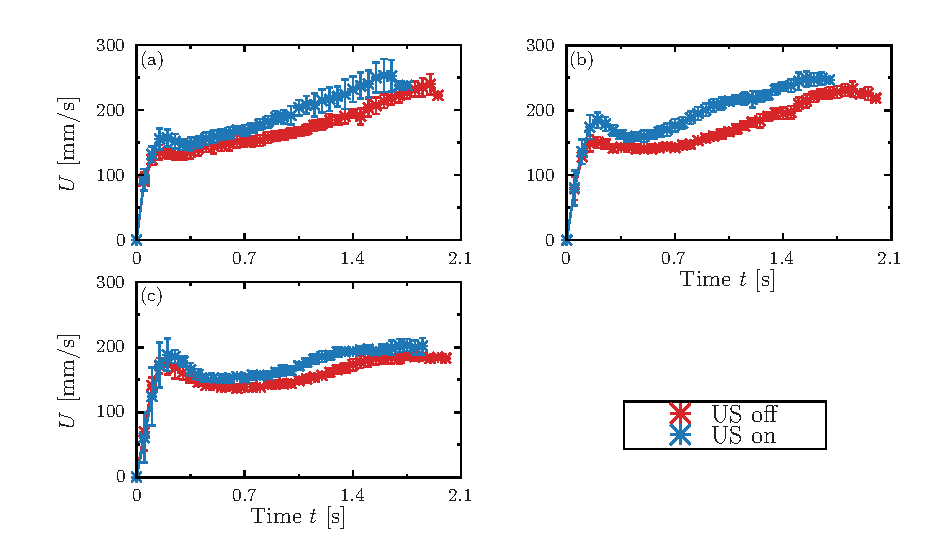
\includegraphics[width=1\textwidth]{./X-Appendix/interval/interval.eps}
    \caption{Falling speed of a sphere in 1wt.\%PAA solution with and without ultrasound irradiation for the interval (a)5min, (b)10min, (c)20min.)}
    \label{fig:falling-interval}
\end{figure}

\clearpage

\subsection{超音波照射による高速化}

球の落下間隔を5分,10分,20分と変化させた.その結果をFig.\ref{fig:interval-change}に示す.なお,縦軸は落下速度[mm/s],横軸は落下開始時からの経過時間[s]である.全ての条件において超音波照射に伴う高速化は見られた.また落下速度は,落下間隔10分,5分,20分の順で速かった.この結果を元に,超音波照射時の球の落下速度$U_{on}$と超音波照射なしの球の落下速度$U_{off}$として,速度比$U_{on}/U_{off}$を求めた.その結果をFig.\ref{fig:speed-diff}に示す.ここで縦軸は速度比[-],横軸は落下間隔時間[min]である.この結果より,落下速度と同様に,落下間隔10分,5分,20分の順で超音波照射による高速化が見られた.これに関して,超音波照射による高速化のメカニズムより考える.

今回,落下間隔を変化させたが,音響圧$\Delta P$,水溶液密度$\rho_1$,音速$c$,周波数$f$はすべて同一であった.よって,$k,n$ の2つがパラメータとして考えられる.Iwamuro\cite{ref:9}における擬塑性流体の経時変化や濃度変化における粘性特性の変化\cite{ref:Rahimi2007},\cite{ref:Agi2018} より,$n$よりも$k$の方がパラメータとして大きく作用することが分かる.よって,$k$のみをパラメータとして扱うと,速度比$U_{ABL}/U_0$は,$k^\frac{n}{n+1}$によって変化することが分かる.ここで,$n=0.24$とすると,$\delta \propto k^{0.19}$となり,境界層厚さは粘度定数に対して単調増加する.また,式(\ref{eq:power-law})より,$k$が増加すると粘度$\mu$は大きくなり,式(\ref{eq:UT})より落下速度は遅くなることも分かる.ゆえに,粘度が大きくなると落下速度が遅くなり,境界層厚さが厚くなる.

今回,落下間隔を変化させた実験結果をFig.\ref{fig:interval-change}に示す.縦軸は落下速度,横軸は落下開始時刻からの経過時間である.この図に示される様に,超音波照射なしでの落下速度は落下間隔10分,5分,20分の順で速かった.これは,落下間隔の変化で流体の粘弾性特性が変化したためだと考えられる.式(\ref{eq:UT})より,落下間隔10分よりも20分の方のが$k$が大きくなり,粘性が大きくなったと考えられる.超音波照射による落下速度を超音波照射なしにおける速度$U_{OFF}$で規格化した落下間隔ごとの結果をFig.\ref{fig:speed-diff}に示す.超音波照射による高速化も,超音波照射なしの落下速度と同様の順で大きくなった.

Iwamuro\cite{ref:8}において,音響境界層内の粘度とその厚さが超音波照射による高速化の要因と示されていた.今回の実験結果において,音響境界層内粘度および厚さの影響(式(\ref{eq:Udiff}))をFig.\ref{fig:speed-diff-iwamuro}に示す.縦軸は超音波照射ありの場合の終端速度$U_{ON}$を,超音波照射なしの場合の終端速度$U_{OFF}$で規格化したものである.横軸は,$\mu_U$を音響境界層内の粘度$\mu_{ABL}$で規格化し,球半径$a$で規格化し音響境界層厚さ$\delta$を乗じたものである.この図に,本実験の結果だけではなくIwamuro\cite{ref:8}の結果も示す.図において,今回の落下間隔を変化させた実験結果は,単調減少となっている.一方でIwamuro\cite{ref:8}の結果と合わせると,誤差バーの範囲内に存在している.音響境界層内の粘度とその厚さが超音波照射による高速化の要因と示されていた.落下間隔を変化させた場合においても同様に,音響境界層内の粘度とその厚さが超音波照射による高速化の要因となっていることが分かる.

今回は粘性による影響を考えた.一方,落下開始時のオーバーシュートが落下間隔20分の場合のみ見られ,落下間隔を長くすると弾性による影響を受けることも分かる.このため粘性だけではなく,弾性による影響を考慮する必要があるということが考えられる.これを解明するために,それぞれの落下間隔における貯蔵弾性率の計測等も行う必要があると考えられる.

\begin{figure}[ht]
    \begin{center}
        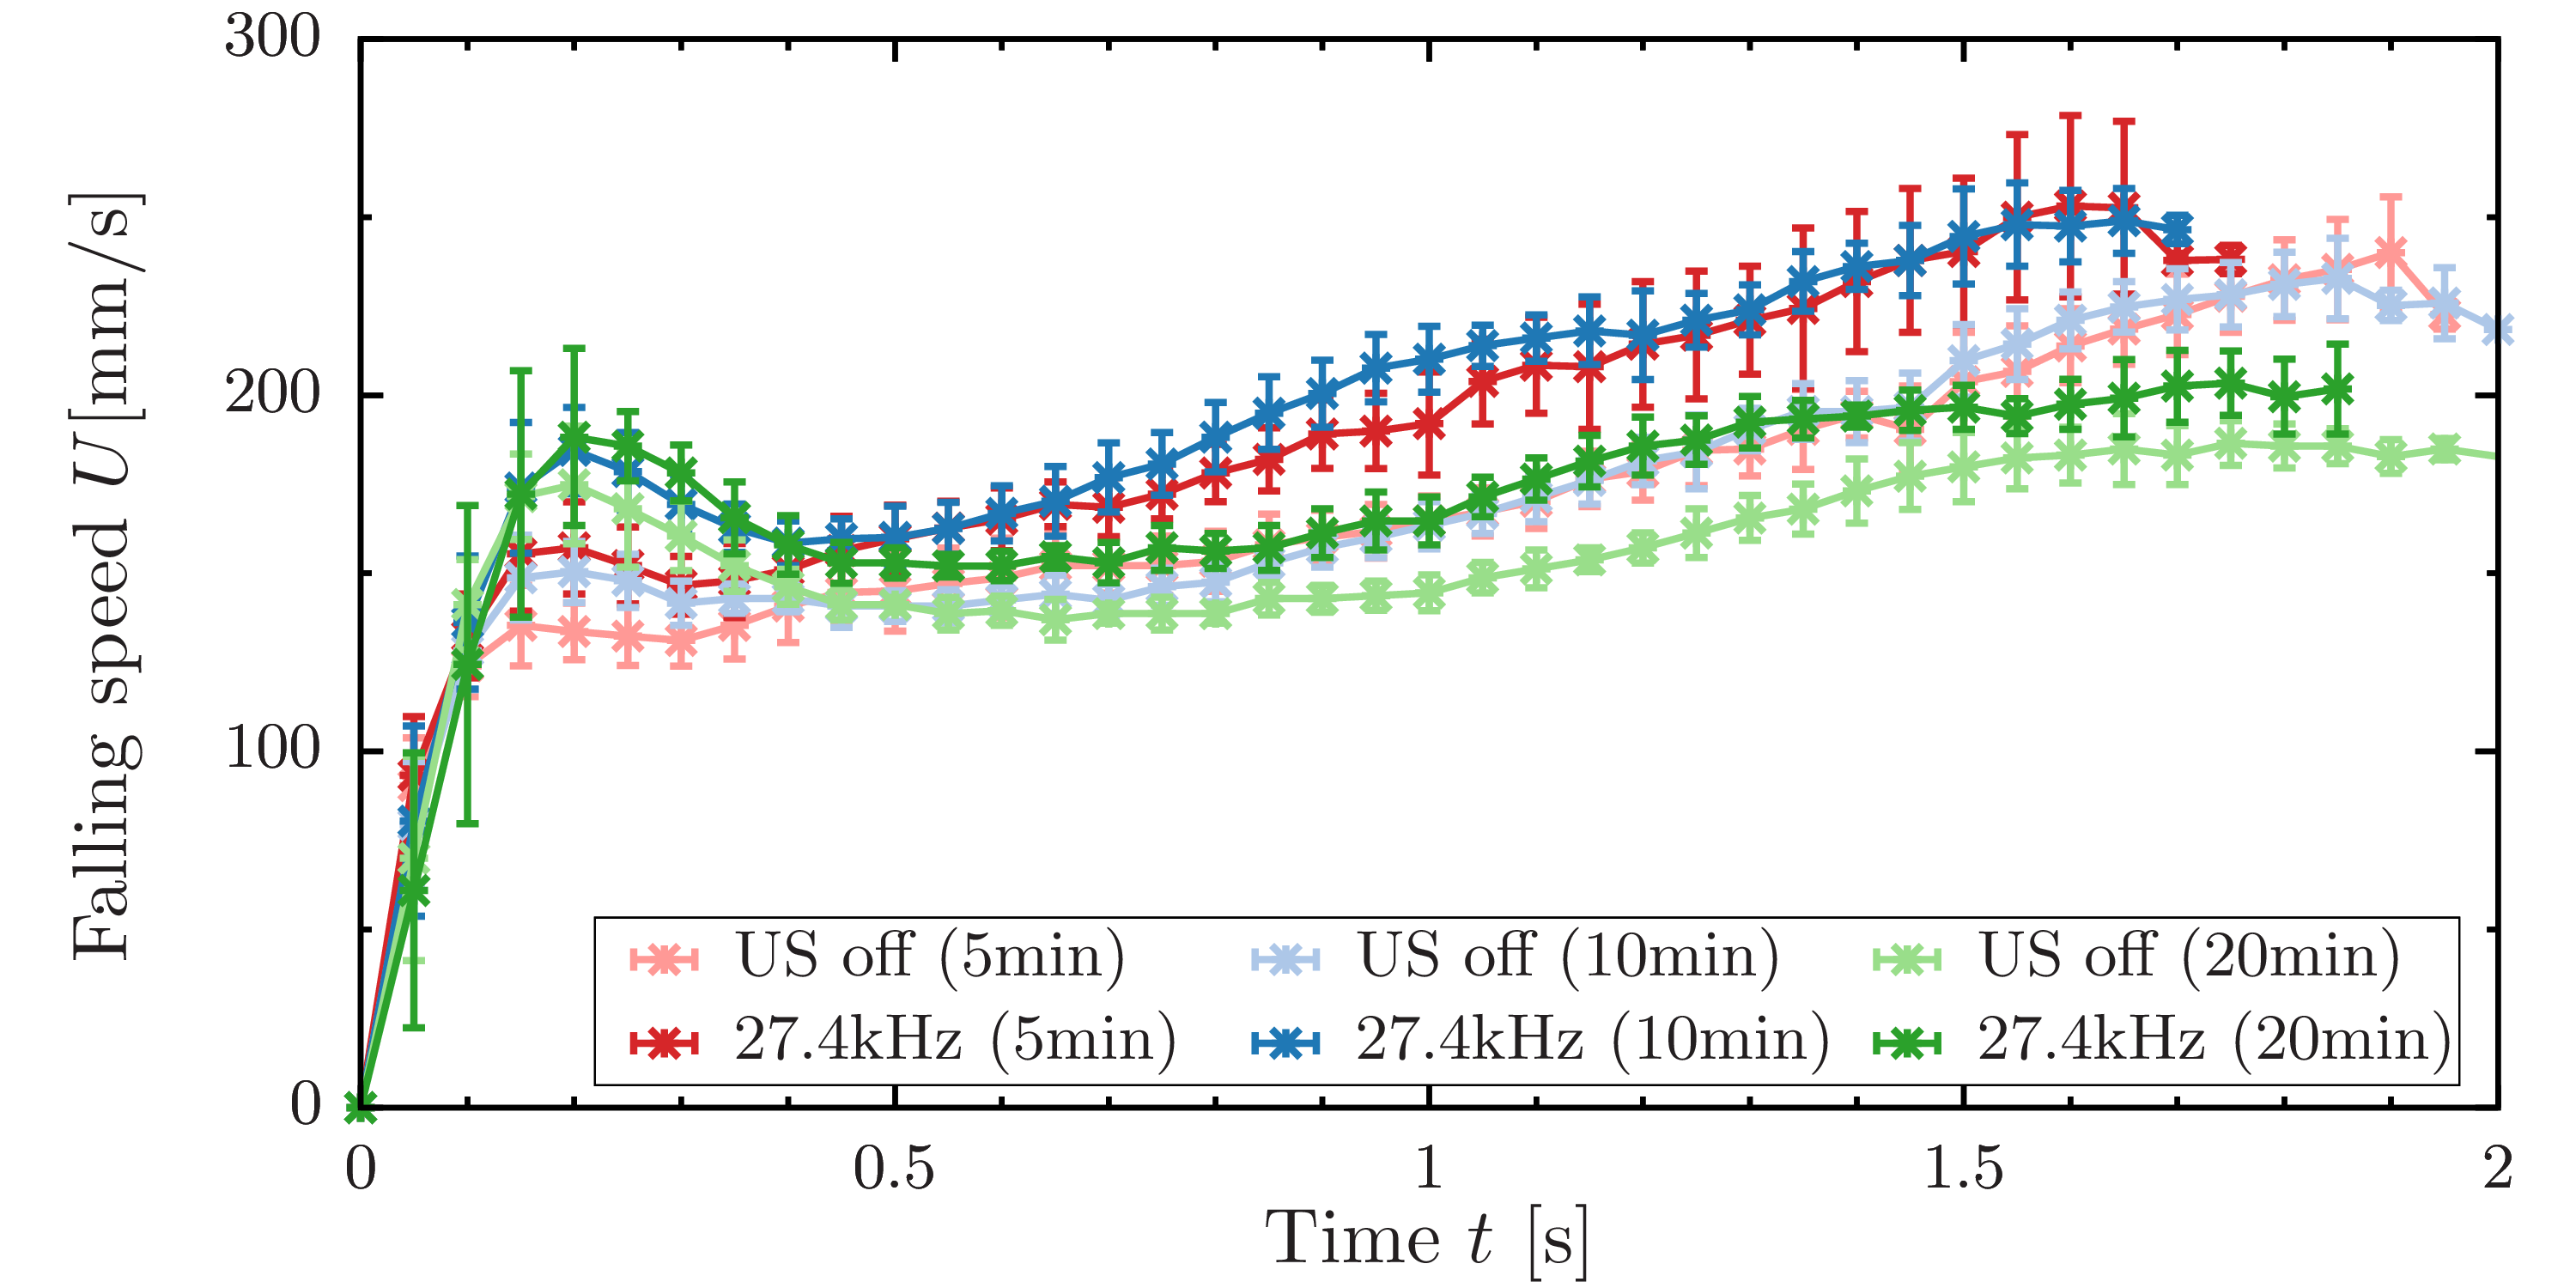
\includegraphics[width=13cm,clip]{5-Results/interval.png}
        \caption{Drop interval change Experimental results.}
        \label{fig:interval-change}
    \end{center}
\end{figure}

\begin{figure}[ht]
    \begin{center}
        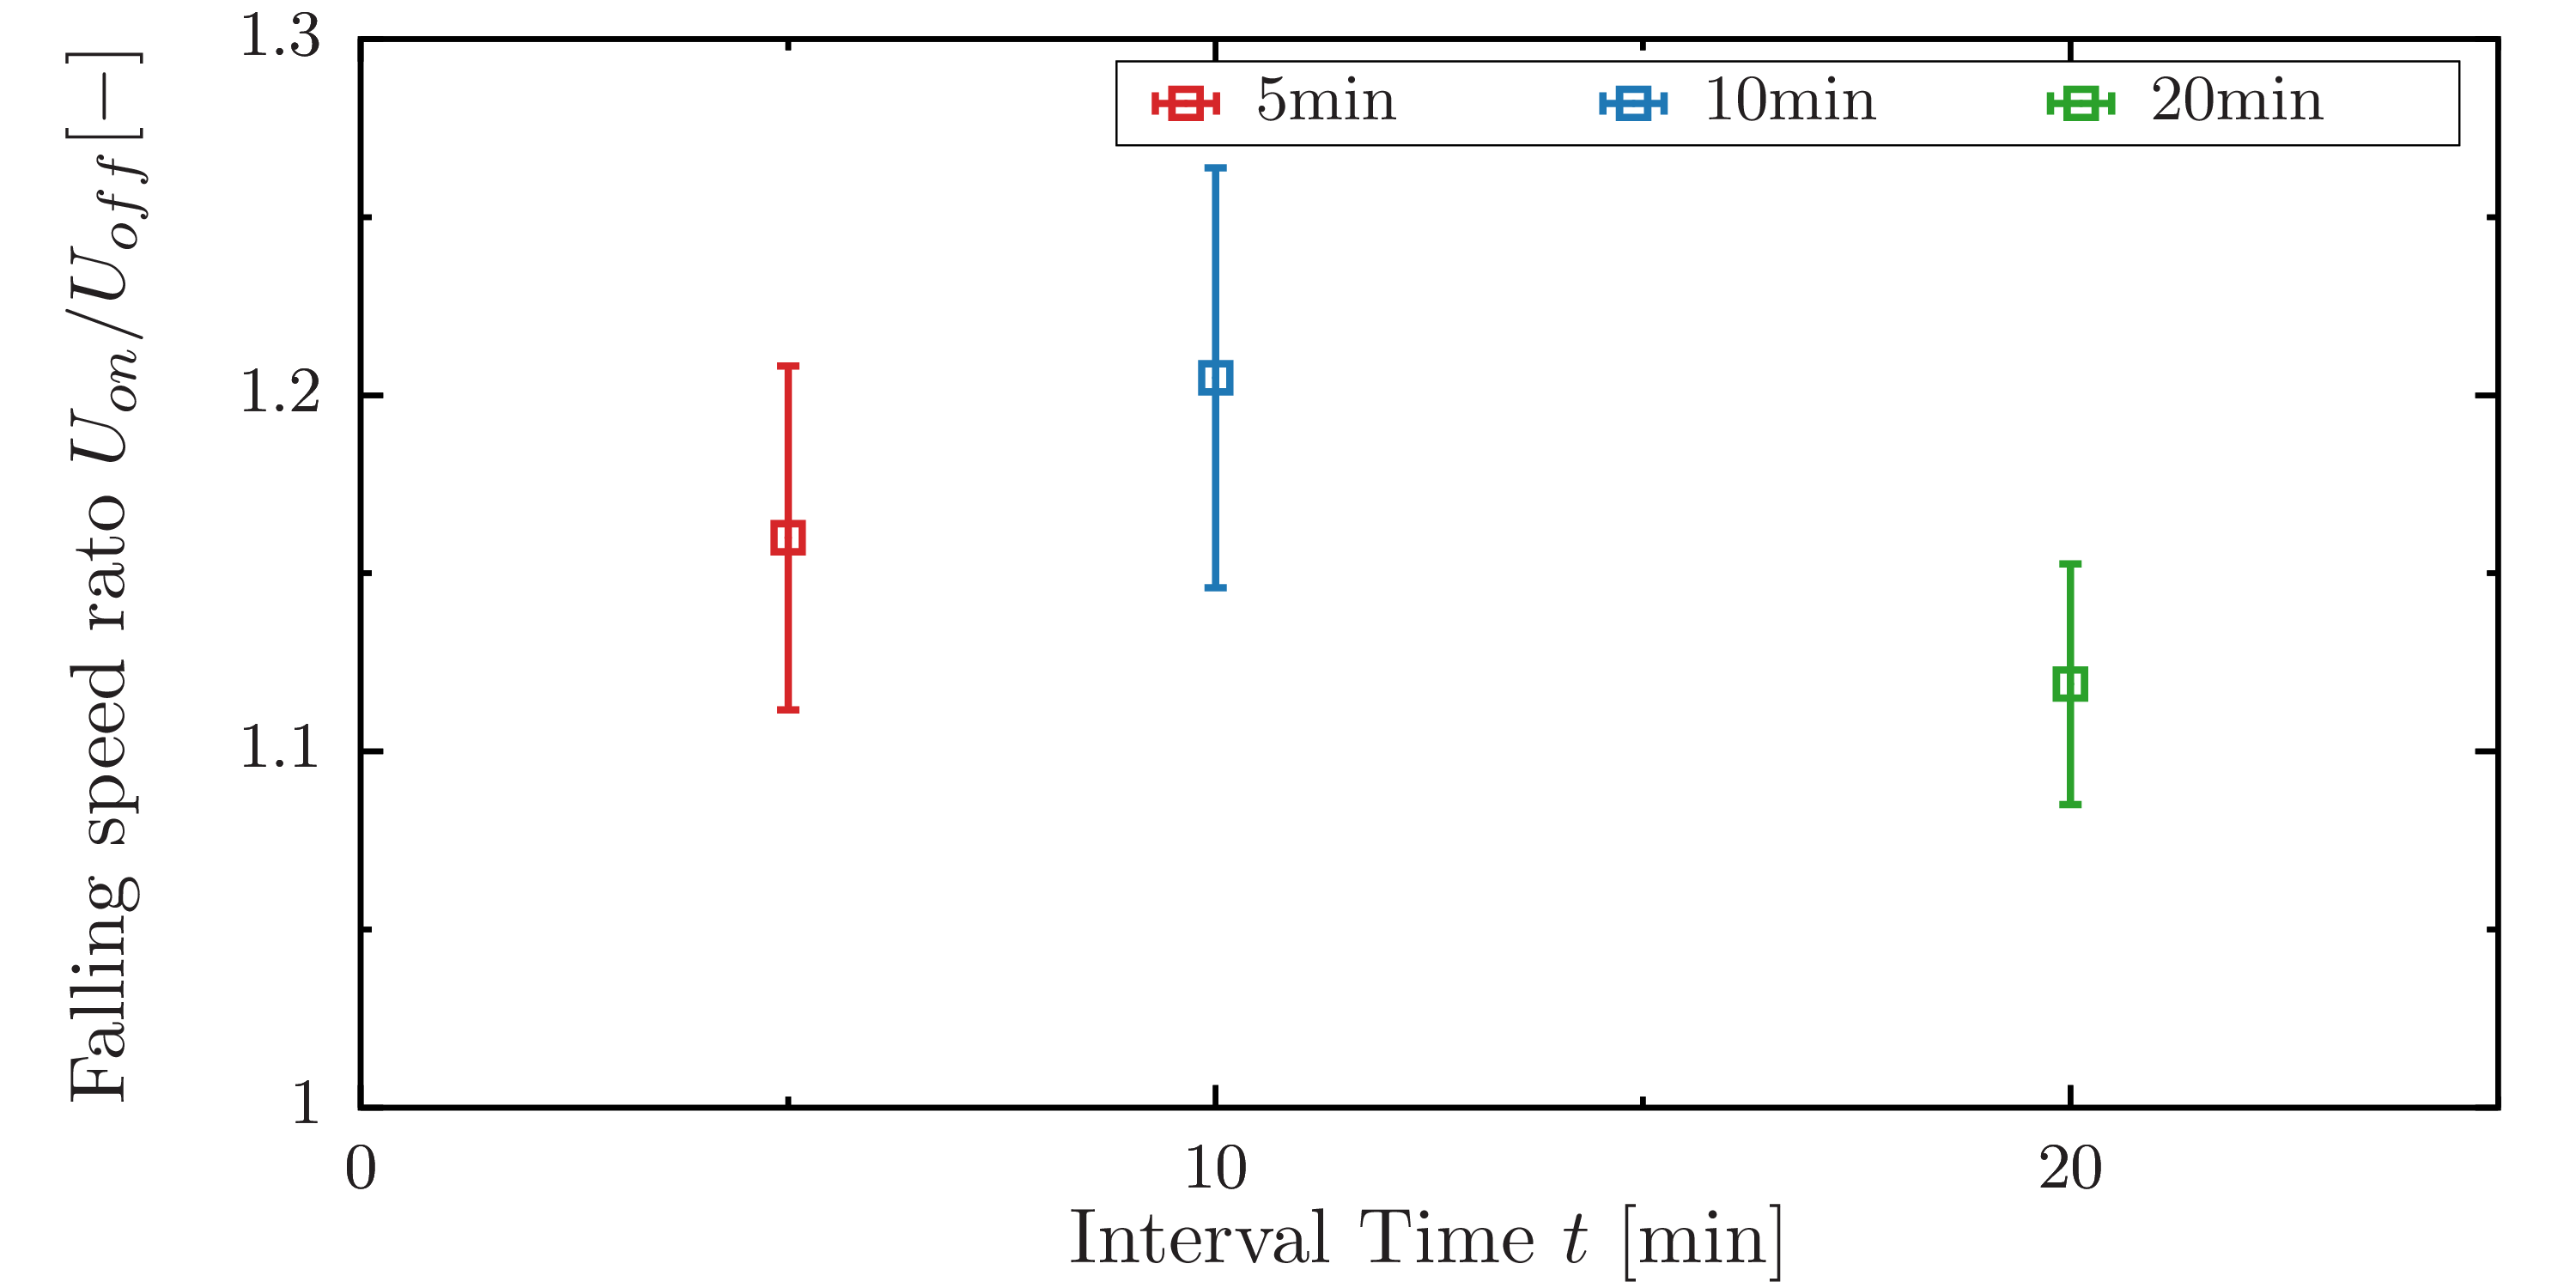
\includegraphics[width=13cm,clip]{5-Results/diff.png}
        \caption{Falling speed ratio due to ultrasound irradiation with change in fall interval.}
        \label{fig:speed-diff}
    \end{center}
\end{figure}

\begin{figure}[ht]
    \begin{center}
        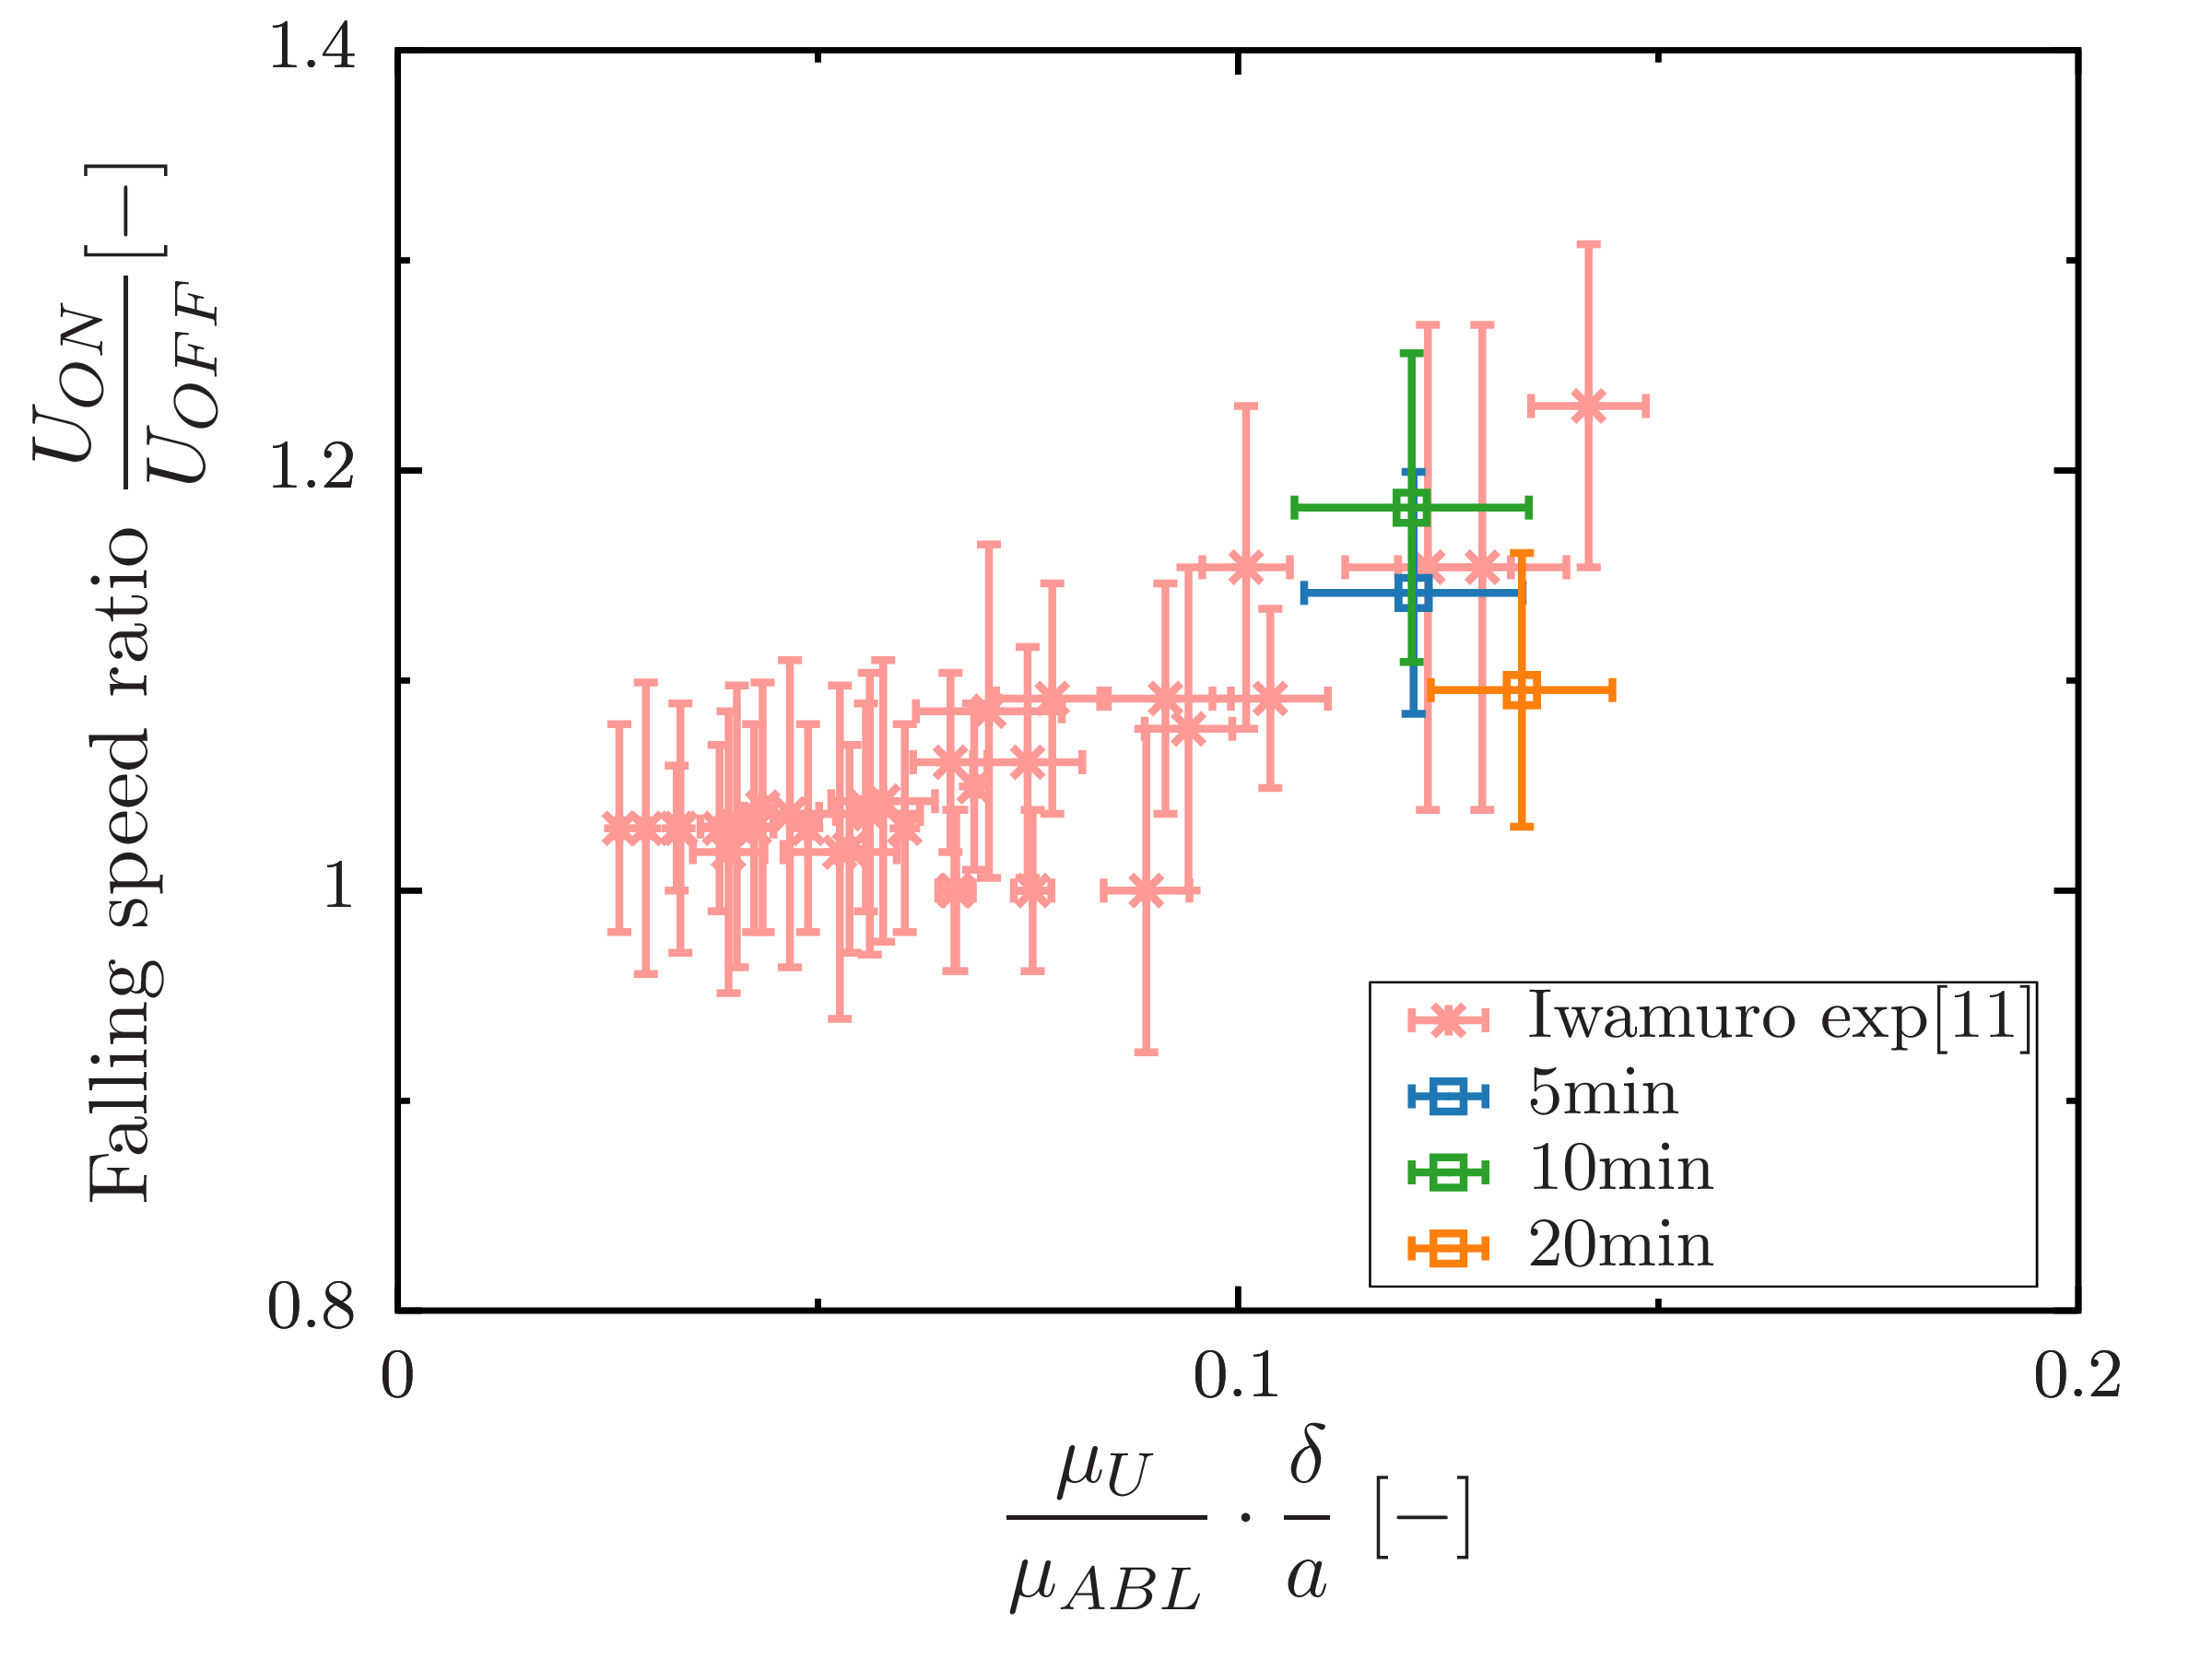
\includegraphics[width=13cm,clip]{5-Results/diff-iwamuro.png}
        \caption{Relationship between viscosity and its thickness in the acoustic boundary layer and speed-up by ultrasound irradiation.}
        \label{fig:speed-diff-iwamuro}
    \end{center}
\end{figure}